%TCIDATA{LaTeXparent=0,0,relatorio.tex}



\chapter{Análise de Dados} \label{chap:Resultados}

% Resumo opcional. Comentar se não usar.
\resumodocapitulo{``Analisar os dados tops!'' -- Tiago}


\section{Introdução}

Nesse capítulo iremos explicar um pouco melhor os experimentos realizados, descritos na seção \ref{section:TestesRealizados}. Iremos também mostrar seus resultados e analisá-los. Lembrando que os experimentos realizados foram:

\begin{itemize}
	\item Apendizagem de 3 comportamentos em um mapa pequeno
	\item Apendizagem de 3 comportamentos no mapa clássico
	\item Apendizagem de 5 comportamentos em um mapa pequeno
	\item Apendizagem de 5 comportamentos no mapa clássico
\end{itemize}

\section{3 Comportamentos no mapa pequeno}

Nesse experimento%
\footnote{Os parâmetros e o setup desse experimento estão melhor descritos no tópico \ref{subsection:3ComportamentosMapaPequeno}.%
} utilizamos apenas 3 comportamentos, $ B = \{Ficar\_Parado, Comer, Fugir\} $, e usamos como vetor de características $ f $, sendo ele:

\begin{equation}
	\begin{array}{r l}
		Bias: & f_1 \left( a, u \right) = 1.0 \\
		Dist Comida: & f_2 \left( a, u \right) = ObterCaracteristicaDistanciaComida \left( a \right) \\
		Prob. Fantasma: & f_3 \left( a, u \right) = ObterCaracteristicaProbFantasmas \left( a \right)
	\end{array}
\end{equation}

Realizamos o treinamento ao longo de 2700 partidas, sendo que a exploração gulosa (\textit{greedy exploration}) foi executada até a partida 1500. Após terminado o treinamento utilizamos 300 partidas para avaliar e obter dados sobre o algoritmo treinado.


\subsection{Resultados e Análise}

A evolução da aprendizagem se dá a partir da mudança dos pesos $ \omega_i $ ao longo do tempo, devido à sua relação com o comportamento selecionado via a equaçào \ref{equation:QLearningEscolhaComportamentoFinal}. Nas figuras \ref{img:3ComportamentosMapaPequeno:PesoBias}, \ref{img:3ComportamentosMapaPequeno:PesoDistComida}, \ref{img:3ComportamentosMapaPequeno:PesoProbFantasma} temos os gráficos de como os valores desses pesos evoluem com o tempo, para cada um dos comportamentos.

\begin{figure}[H]
    \centering
    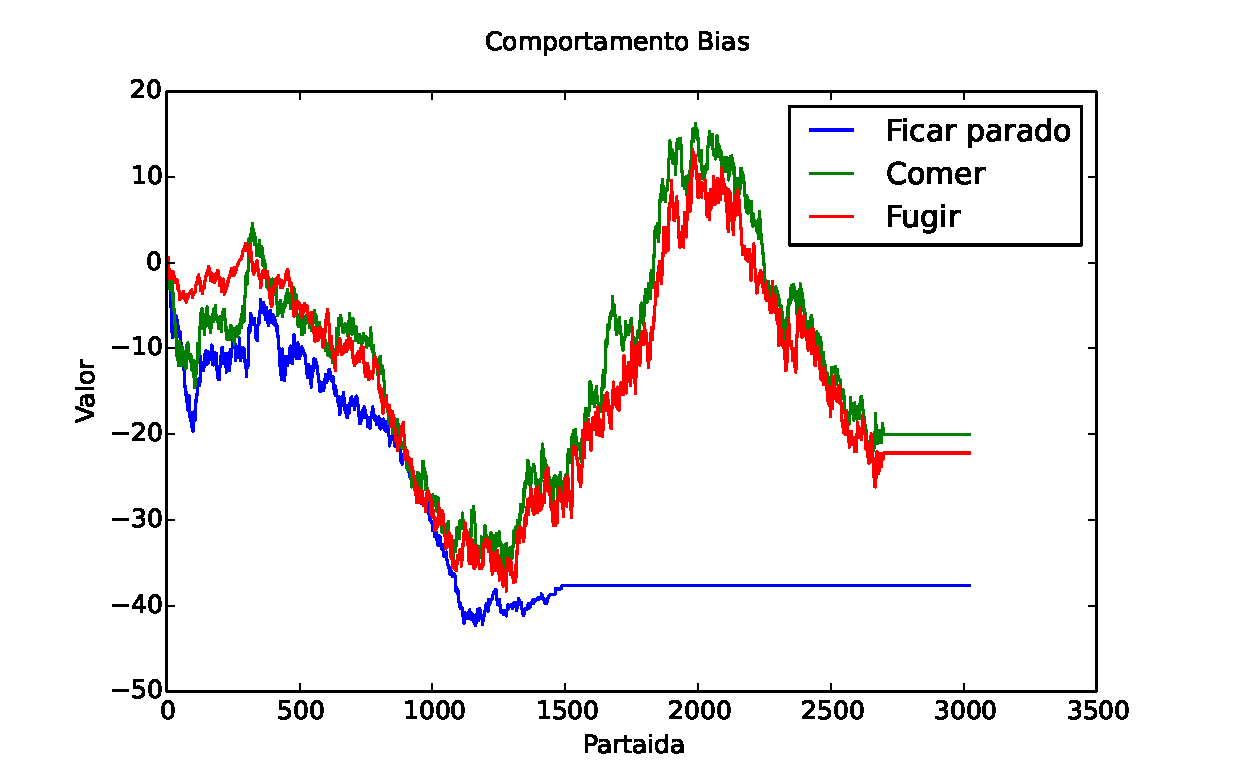
\includegraphics[width=\linewidth]{images/3_behaviors_small_map/weights____pol__Bias}
    \caption{Evolução dos pesos $ \omega_1 $ da característica Bias $ f_1 $.}
    \label{img:3ComportamentosMapaPequeno:PesoBias}
\end{figure}

\begin{figure}[H]
    \centering
    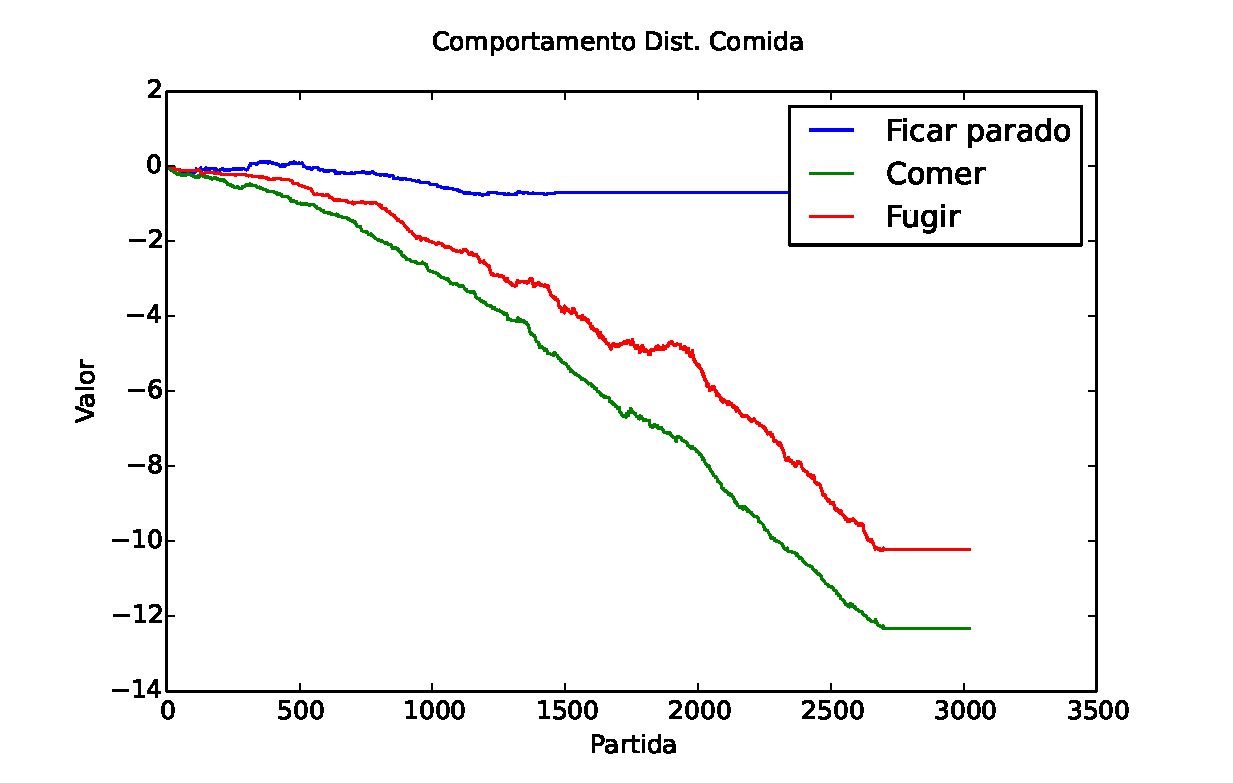
\includegraphics[width=\linewidth]{images/3_behaviors_small_map/weights____pol__DistComida}
    \caption{Evolução dos pesos $ \omega_2 $ da característica Distância para Comida $ f_2 $.}
    \label{img:3ComportamentosMapaPequeno:PesoDistComida}
\end{figure}

\begin{figure}[H]
    \centering
    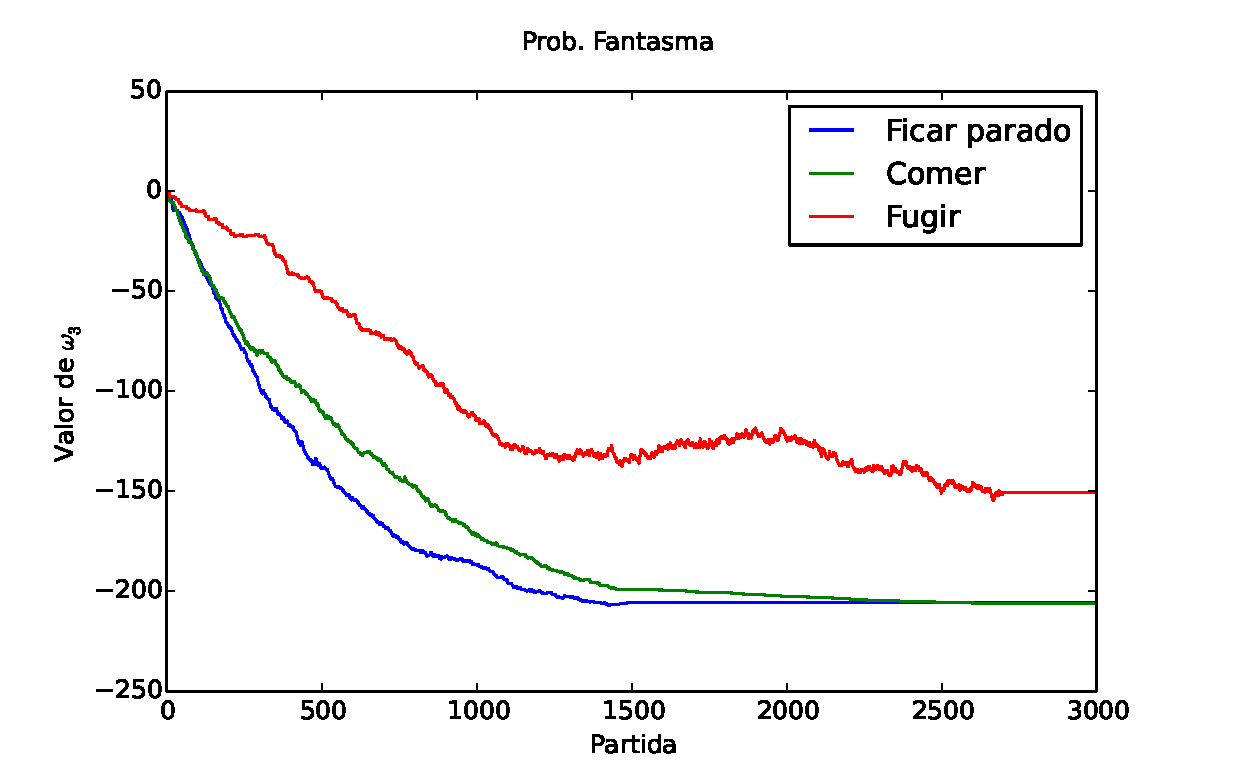
\includegraphics[width=\linewidth]{images/3_behaviors_small_map/weights____pol__ProbFantasma}
    \caption{Evolução dos pesos $ \omega_3 $ da característica Probabilidade de Fantasma $ f_3 $.}
    \label{img:3ComportamentosMapaPequeno:PesoProbFantasma}
\end{figure}

É fácil notar que o peso $ \omega_3 $, relativo à carascterística probabilidade de haver um fantasma normal perto, $ f_3 $, é o que cresce mais rápido e que atinge valor absoluto final maior, entre -140 e -210, enquanto os outros dois ficam entre -50 e 20. Isso acontece pois ele sempre tem um valor alto quando o pacman é morto, recebendo uma recompensa de -500 pontos. Quando os pesos são atualizados, seguindo as equações \ref{equation:ErroQPartiallyObservable} e \ref{equation:UpdateOmegaQPartiallyObservable}, esse peso será bastante modificado a cada morte do pacman. Isso mostra também que ele aprende que essa é uma situação ruim, dando um valor menor para estados em que ela tem valor mais alto ($ \uparrow f_3 \rightarrow \downarrow \downarrow Q $).

Outro fato ressaltado por esses gráficos é que estar perto de fantasmas é menos ruim no caso de se escolher o comportamento fugir, do que para comer ou ficar parado. Analisando esses valores é possível ver que o comportamento $ Ficar\_Parado $ nunca será executado%
\footnote{Lembrando que, como explicado no tópico \ref{subsection:3ComportamentosMapaPequeno}, o valor de $ f_2 \left( A, B \right) $ estará sempre entre 0 e 1.%
}, o comportamento $ Comer $ será o normalmente utilizado e o comportamento $ Fugir $ será utilizado quando a probabilidade de haver um fantasma por perto for alta.

Qual comportamento é escolhido a cada instante e quantas vezes cada um é escolhido por partida são fatores importantes para avaliar esse algoritmo. Quando pegamos o número de vezes que cada comportamentos é escolhido por partida e plotamos esses dados como pontos num gráfico eles formam a seguinte nuvem, exposta na figura \ref{img:3ComportamentosMapaPequeno:ComportamentosEscolhidos}.

\begin{figure}[H]
    \centering
    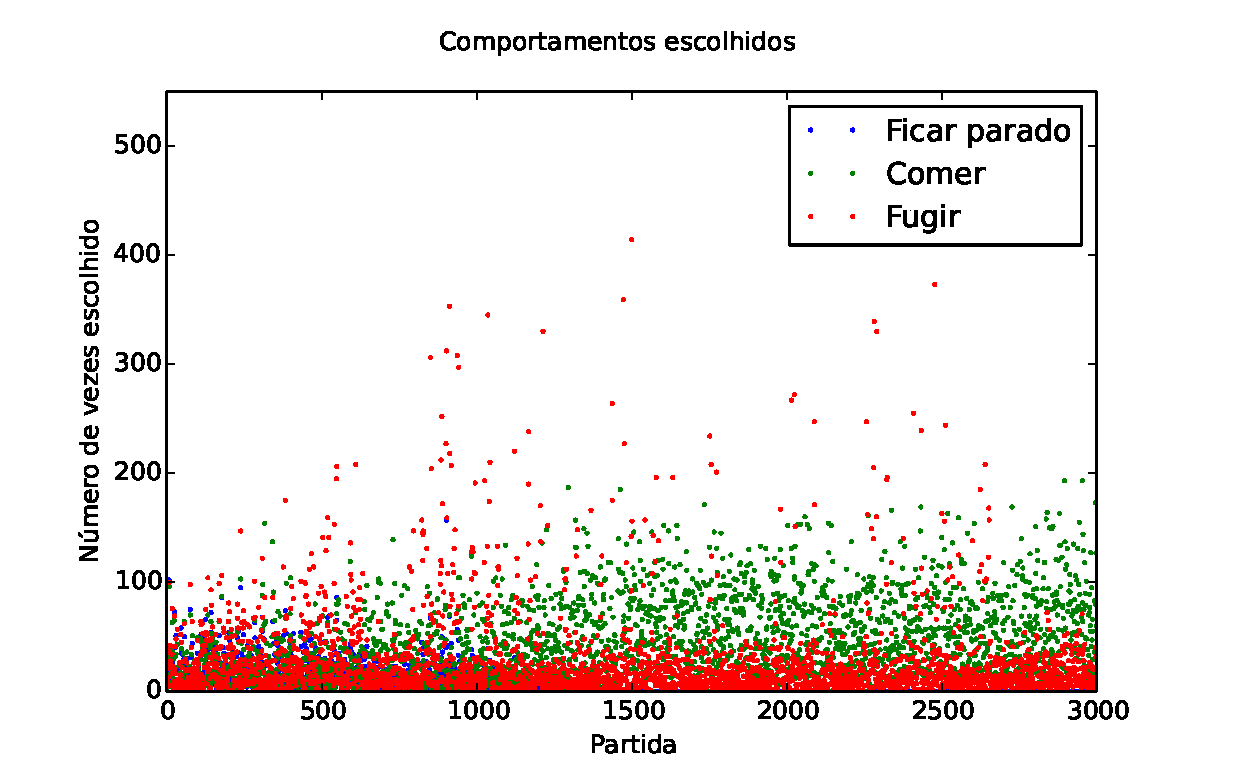
\includegraphics[width=\linewidth]{images/3_behaviors_small_map/chosen_behaviors}
    \caption{Escolha de comportamentos por partida.}
    \label{img:3ComportamentosMapaPequeno:ComportamentosEscolhidos}
\end{figure}

Com essa nuvem de dados já podemos começar a avaliar como essa escolha de comportamento é feita ao longo do tempo, mas para ter uma visualização melhor podemos aproximar um polinômio dessa nuvem de pontos, utilizando o método dos mínimos quadrados. Para um polinômio de quarto grau essa curva fica como a descrita na figura \ref{img:3ComportamentosMapaPequeno:ComportamentosEscolhidosPolinômio}.

\begin{figure}[H]
    \centering
    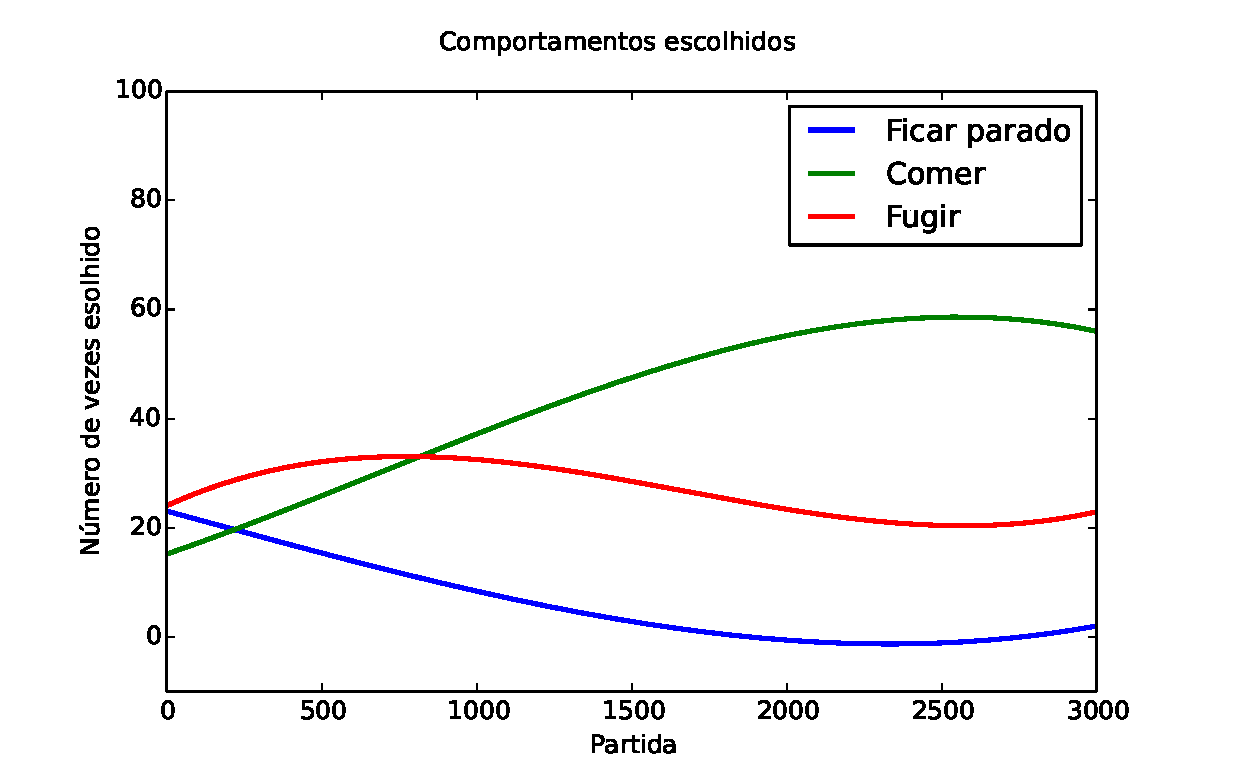
\includegraphics[width=\linewidth]{images/3_behaviors_small_map/chosen_behaviors_pol}
    \caption{Escolha de comportamentos por partida.}
    \label{img:3ComportamentosMapaPequeno:ComportamentosEscolhidosPolinômio}
\end{figure}

Inicialmente o comportamento $ Comer $ diminui em números de execução, enquanto $ Fugir $ aumenta. Isso acontece porque, inicialmente, não sabendo nada sobre o mundo, o agente ``percebe'' que quando ele executa o comportamento $ Comer $, ele tem muito mais probabilidade de morrer. Após aproximadamente 500 partidas, percebemos que esse comportamento começa a aumentar em número de execuções, enquanto o $ Fugir $ diminui.

Outro dado relevante para a análise é a pontuação obtida por jogo, que tentamos otimizar ao dá-la como recompensa para nossa função de treinamento. A pontuação para cada partida pode ser vista na imagem \ref{img:3ComportamentosMapaPequeno:PontuacaoPorPartida}, à seguir. Assim como para a evolução dos comportamentos escolhidos ao longo do tempo, também aproximamos esses dados por um polinômio, dessa vez de terceiro grau, utilizando o método dos mínimos quadrado.

\begin{figure}[H]
    \centering
    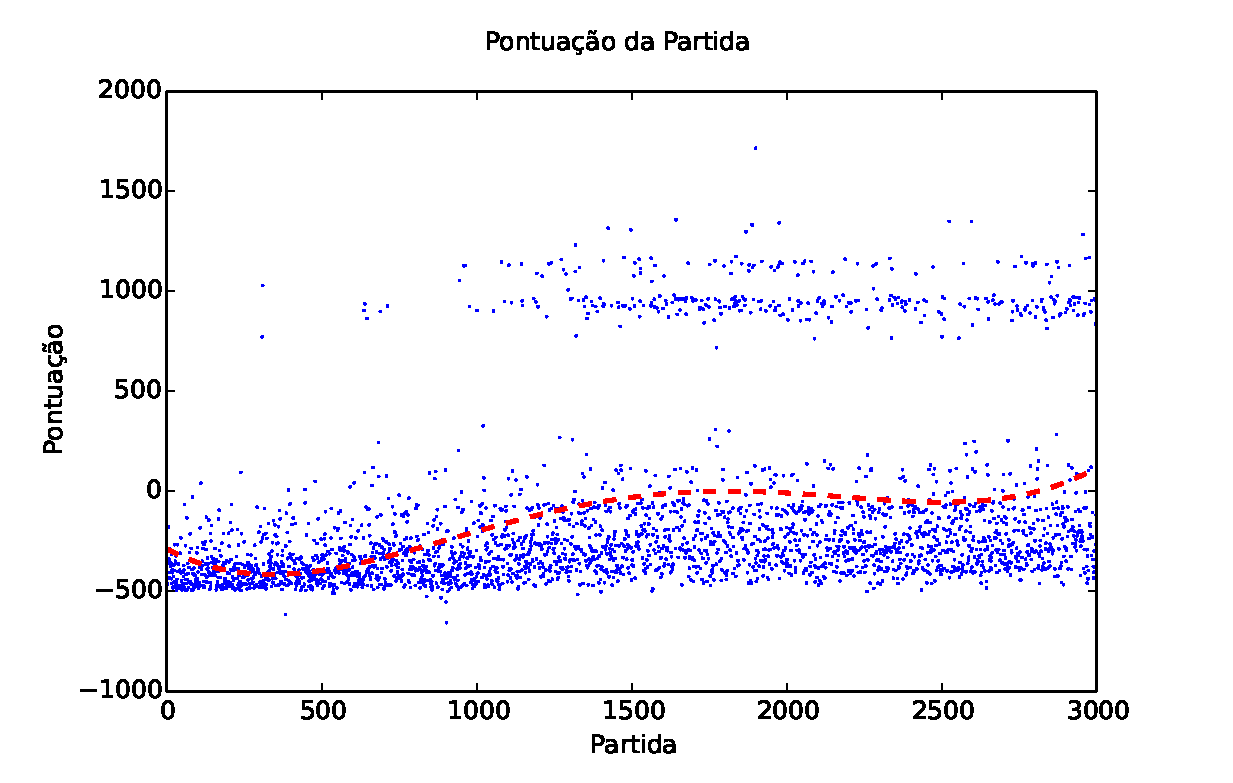
\includegraphics[width=\linewidth]{images/3_behaviors_small_map/match_scores____pol}
    \caption{Escolha de comportamentos por partida.}
    \label{img:3ComportamentosMapaPequeno:PontuacaoPorPartida}
\end{figure}

É possível perceber que essa função é ascendente e que segue, aproximadamente, o formato da curva do número de execuções do comportamento $ Comer $. Isso acontece pois, inicialmente, ao aumentar o número de execuções de $ Fugir $, se diminui a pontuação geral%
\footnote{Se não pegar uma comida, se perde um ponto por movimento.%
}. A média de pontos feita, após a conclusão do treinamento:

$$ mean \left( score \right) =50.04 $$

Sendo a média de escolha pelo algorítmo de aprendizagem dos comportamentos:

$$ mean \left( Ficar\_Parado \right) = 0.0 $$
$$ mean \left( Comer \right) = 61.77 $$
$$ mean \left( Fugir \right) = 17.21 $$


\subsection{Discussão}

Podemos ver que o algoritmo teve o resultado esperado para esse mapa e esses comportamentos, escolhendo sempre fugir, quando tendo alta probabilidade de perigo por perto, e comer no caso contrário.


\section{3 Comportamentos no mapa original (Teste 2)}

Nesse experimento%
\footnote{Os parâmetros e o setup desse experimento estão melhor descritos no tópico \ref{subsection:3ComportamentosMapaOriginal}.%
}, assim como no anterior, utilizamos apenas 3 comportamentos, $ B = \{Ficar\_Parado, Comer, Fugir\} $, e usamos como vetor de características $ f $, sendo ele:

\begin{equation}
	\begin{array}{r l}
		Bias: & f_1 \left( a, u \right) = 1.0 \\
		Dist Comida: & f_2 \left( a, u \right) = ObterCaracteristicaDistanciaComida \left( a \right) \\
		Prob. Fantasma: & f_3 \left( a, u \right) = ObterCaracteristicaProbFantasmas \left( a \right)
	\end{array}
\end{equation}

Realizamos o treinamento ao longo de 700 partidas, sendo que a exploração gulosa (\textit{greedy exploration}) foi executada até a partida 500. Após terminado o treinamento utilizamos 300 partidas para avaliar e obter dados sobre o algoritmo treinado.


\subsection{Resultados e Análise}

Como no experimento anterior, nas figuras à seguir \ref{img:3ComportamentosMapaOriginal:PesoBias}, \ref{img:3ComportamentosMapaOriginal:PesoDistComida}, \ref{img:3ComportamentosMapaOriginal:PesoProbFantasma} temos os gráficos de como os valores dos pesos $ \omega_i $ evoluem com o tempo, para cada um dos comportamentos.

\begin{figure}[H]
    \centering
    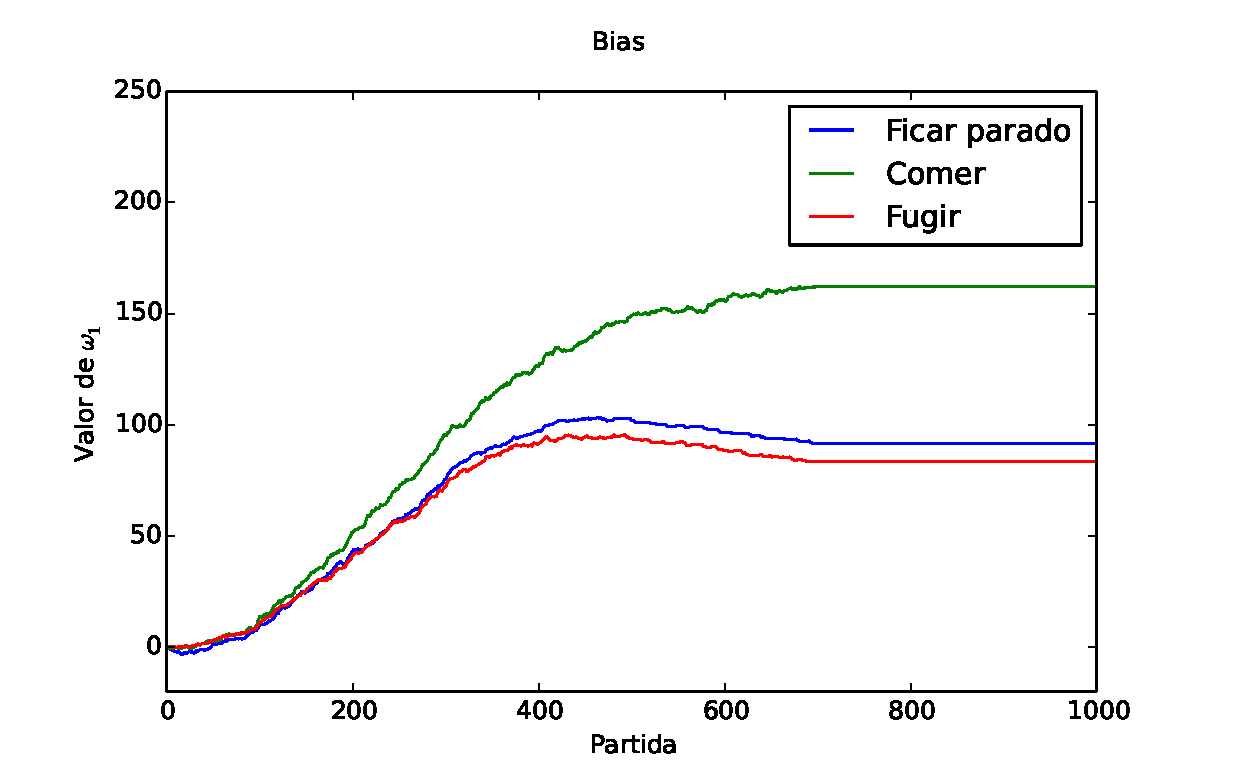
\includegraphics[width=\linewidth]{images/3_behaviors_original_map/weights____pol__Bias}
    \caption{Evolução dos pesos $ \omega_1 $ da característica Bias $ f_1 $.}
    \label{img:3ComportamentosMapaOriginal:PesoBias}
\end{figure}

\begin{figure}[H]
    \centering
    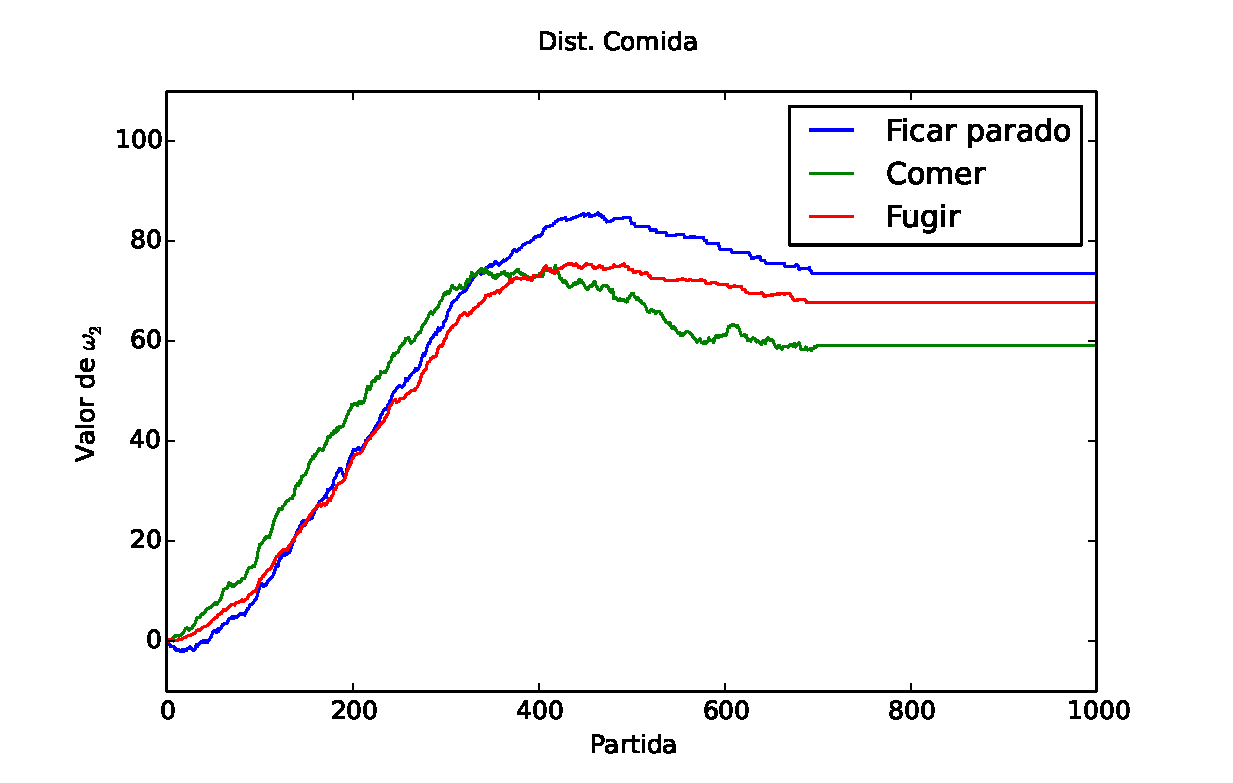
\includegraphics[width=\linewidth]{images/3_behaviors_original_map/weights____pol__DistComida}
    \caption{Evolução dos pesos $ \omega_2 $ da característica Distância para Comida $ f_2 $.}
    \label{img:3ComportamentosMapaOriginal:PesoDistComida}
\end{figure}

\begin{figure}[H]
    \centering
    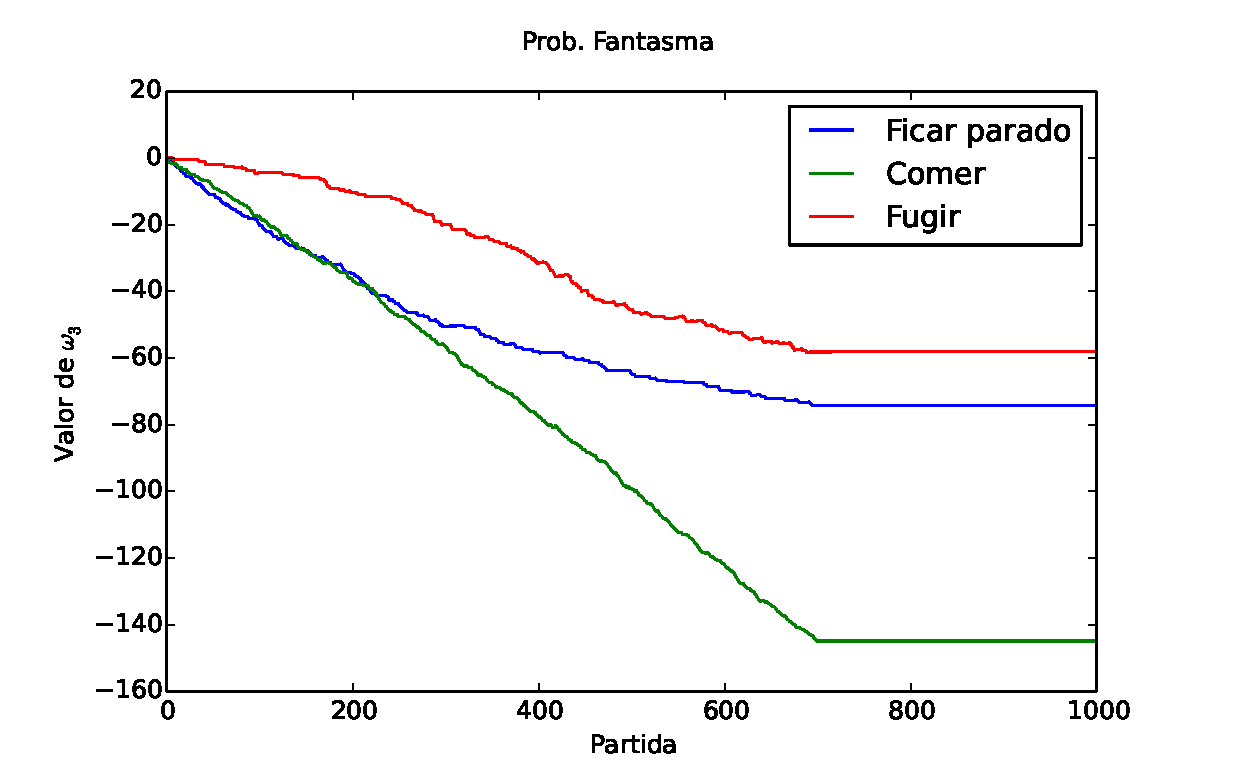
\includegraphics[width=\linewidth]{images/3_behaviors_original_map/weights____pol__ProbFantasma}
    \caption{Evolução dos pesos $ \omega_3 $ da característica Probabilidade de Fantasma $ f_3 $.}
    \label{img:3ComportamentosMapaOriginal:PesoProbFantasma}
\end{figure}

Podemos notar que, para esse experimento, todos os pesos, $ \omega_1 $, $ \omega_2 $ e $ \omega_3 $ , tem valores relativamente altos. Isso se dá, em boa parte, por esse ser um mapa ``fácil''. Como se demora mais para morrer, pois o mapa é grande e se tem menos chance de encontrar um fantasma, o peso da característica $ Prob. Fantasma $ cresce (ou diminui, já que é negativa) mais lentamente. Além disso, como se morre menos vezes, os pesos das outras características tende a aumentar mais do que diminuir.

Novamente, conseguimos reparar que o fato de $ \omega_3 $, o peso de $ Prob.Fantasma $, ser negativo e com valor absoluto alto para o comportamento $ Comer $, mostra que ele aprende que essa é uma situação ruim para se escolher esse comportamento. Também vemos novamente que estar perto de fantasmas é menos ruim no caso de se escolher o comportamento fugir, do que para comer ou ficar parado.

Um fato que pode parecer estranho a primeira vista é o fato de o peso $ \omega_2 $, da característica $ Dist. Comida $, ser maior para ficar parado e menor para comer. Isso ocorre pois os pesos devem se balancear pela equação de calculo do erro \ref{equation:ErroQPartiallyObservable} e, como $ Comer $ tem um peso $ \omega_1 $, da característica $ Bias $, alto, seus outros pesos acabam sendo afetados.

Analisando esses pesos vemos que o comportamento $ Comer $ será o normalmente utilizado, o comportamento $ Fugir $ será utilizado quando a probabilidade de haver um fantasma por perto for alta e o comportamento $ Ficar\_Parado $ será escolhido raramente, quando houver uma probabilidade mediana de haver um fantasma por perto e se estiver perto de uma comida.

Para esse experimento, quando plotamos o número de vezes que cada comportamentos é escolhido por partida como pontos num gráfico eles formam a nuvem exposta na figura \ref{img:3ComportamentosMapaOriginal:ComportamentosEscolhidos}.

\begin{figure}[H]
    \centering
    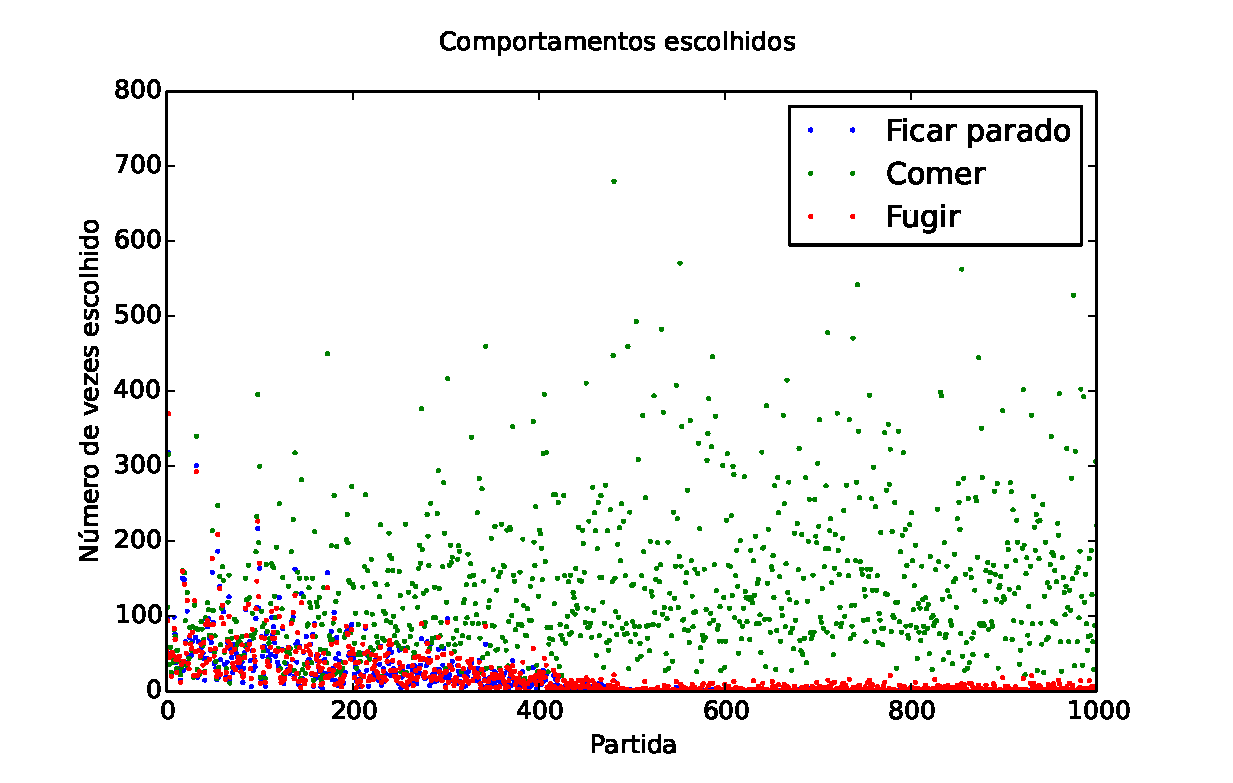
\includegraphics[width=\linewidth]{images/3_behaviors_original_map/chosen_behaviors}
    \caption{Escolha de comportamentos por partida.}
    \label{img:3ComportamentosMapaOriginal:ComportamentosEscolhidos}
\end{figure}

Novamente, para ter uma visualização melhor achamos um polinômio que represente essa nuvem de pontos, utilizando o método dos mínimos quadrados. Para um polinômio de quarto grau essa curva fica como a descrita na figura \ref{img:3ComportamentosMapaOriginal:ComportamentosEscolhidosPolinômio}.

\begin{figure}[H]
    \centering
    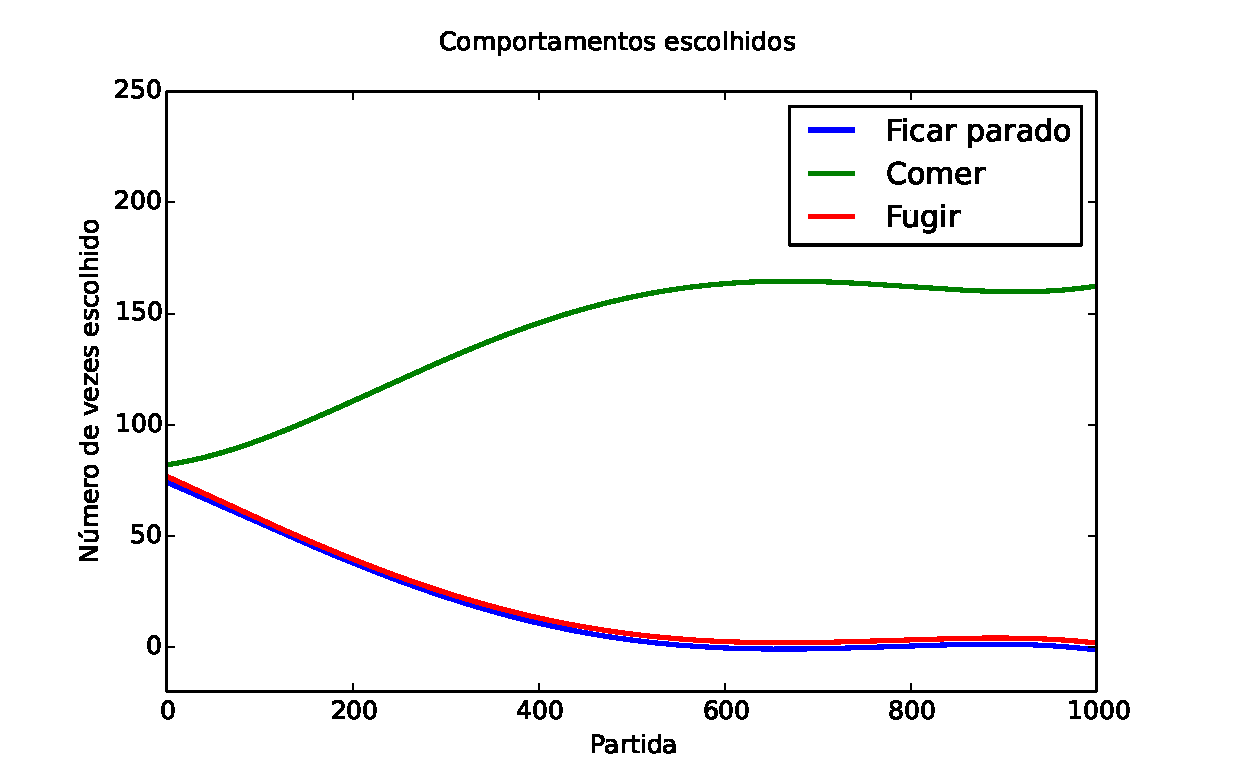
\includegraphics[width=\linewidth]{images/3_behaviors_original_map/chosen_behaviors_pol}
    \caption{Escolha de comportamentos por partida.}
    \label{img:3ComportamentosMapaOriginal:ComportamentosEscolhidosPolinômio}
\end{figure}

Para esse mapa o comportamento $ Comer $ nunca é considerado ruim e sobe em número de execuções rapidamente, enquanto os dois outros $ Comer $ e $ Ficar\_Parado $ diminuem em número de execuções até alcançarem um valor relativamente constante, perto de zero execuções por partida.

A pontuação para cada partida pode ser vista na imagem à seguir, \ref{img:3ComportamentosMapaOriginal:PontuacaoPorPartida}. Novamente aproximamos esses dados por um polinômio de terceiro grau, utilizando o método dos mínimos quadrado.

\begin{figure}[H]
    \centering
    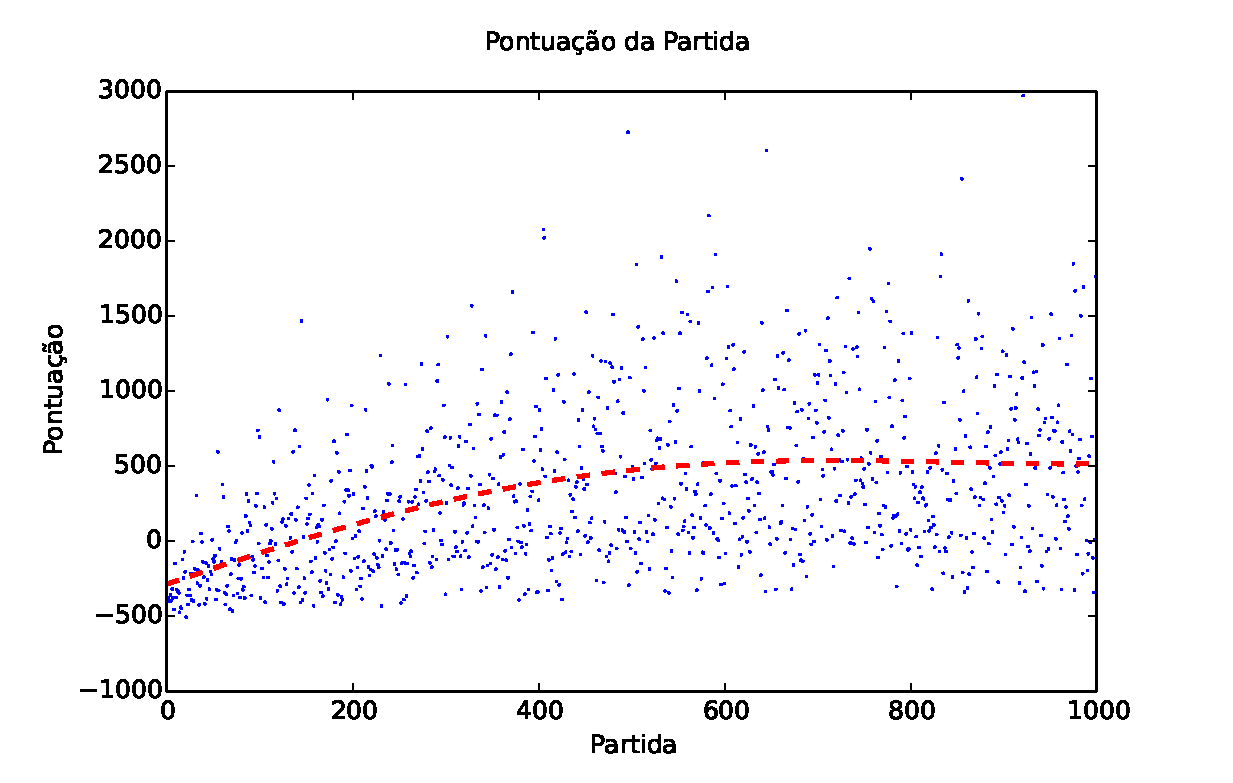
\includegraphics[width=\linewidth]{images/3_behaviors_original_map/match_scores____pol}
    \caption{Escolha de comportamentos por partida.}
    \label{img:3ComportamentosMapaOriginal:PontuacaoPorPartida}
\end{figure}

Essa função é ascendente e tende a uma constante. A média de pontos feita, após a conclusão do treinamento:

$$ mean \left( score \right) = 542.68488746 $$

Sendo a média de escolha pelo algorítmo de aprendizagem dos comportamentos:

$$ mean \left( Ficar\_Parado \right) = 0.183279742765 $$
$$ mean \left( Comer \right) = 164.572347267 $$
$$ mean \left( Fugir \right) = 3.26688102894 $$


\subsection{Discussão}

É possível ver que o algoritmo, nesse experimento, deu preferência à ação de comer, algumas vezes sendo ``super confiante''. Isso é explicado pela facilidade que o agente tem de receber pontos nesse ambiente, tendo mais raro encontro com fantasmas. Além disso, o fato de nesse mapa ele muitas vezes pegar uma Cápsula enquanto está executando a ação de comer, o permitindo comer fantasmas e receber pontos por isso, valoriza essa ação.


\section{5 Comportamentos no mapa pequeno (Teste 3)}

Nesse experimento%
\footnote{Os parâmetros e o setup desse experimento estão melhor descritos no tópico \ref{subsection:5ComportamentosMapaPequeno}.%
}, diferente dos anteriores, utilizamos 5 comportamentos. 

$$ B = \{Ficar\_Parado, Comer, Fugir, Comer\_Cápsula, \textit{Caçar} \} $$

Usamos como vetor de características $ f $:

\begin{equation}
	\begin{array}{r l}
		Bias: & f_1 \left( a, u \right) = 1.0 \\
		Dist. Comida: & f_2 \left( a, u \right) = ObterCaracteristicaDistanciaComida \left( a \right) \\
		Dist. Capsula: & f_3 \left( a, u \right) = ObterCaracteristicaProbFantasmas \left( a \right) \\
		Prob. Capsula Existir: & f_4 \left( a, u \right) = ObterCaracteristicaProbFantasmas \left( a \right) \\
		Prob. Fantasma Branco Existir: & f_5 \left( a, u \right) = ObterCaracteristicaProbFantasmas \left( a \right) \\
		Prob. Fantasma Por Perto: & f_6 \left( a, u \right) = ObterCaracteristicaProbFantasmas \left( a \right) \\
		Prob. Fantasma Branco Por Perto: & f_7 \left( a, u \right) = ObterCaracteristicaProbFantasmas \left( a \right)
	\end{array}
\end{equation}

Realizamos o treinamento ao longo de 2700 partidas, sendo que a exploração gulosa (\textit{greedy exploration}) foi executada até a partida 1500. Após terminado o treinamento utilizamos 300 partidas para avaliar e obter dados sobre o algoritmo treinado.


\subsection{Resultados e Análise}

Nas figuras à seguir, de \ref{img:5ComportamentosMapaPequeno:PesoBias} a \ref{img:5ComportamentosMapaPequeno:PesoProbFantasmaBrancoPorPerto}, temos os gráficos de como os valores dos pesos $ \omega_i $ evoluem com o tempo, para cada um dos comportamentos.

\begin{figure}[H]
    \centering
    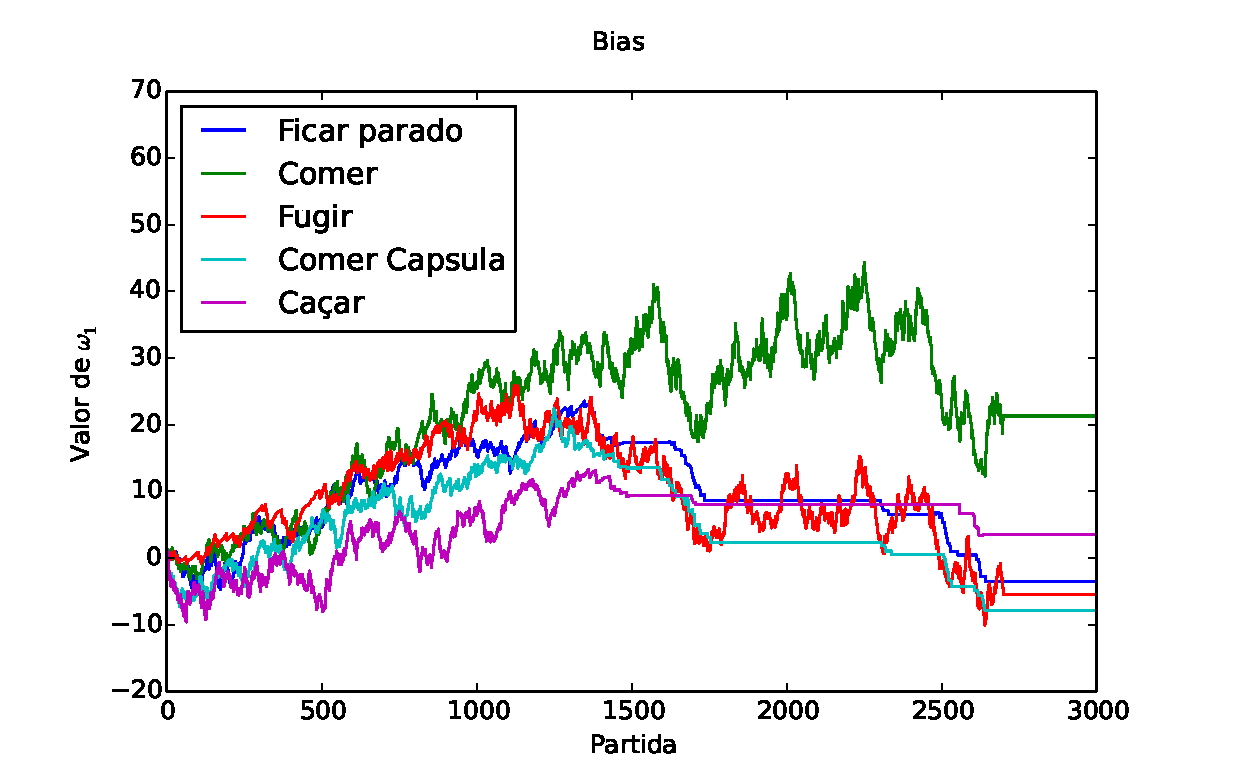
\includegraphics[width=\linewidth]{images/5_behaviors_small_map/weights____pol__Bias}
    \caption{Evolução dos pesos $ \omega_1 $ da característica Bias $ f_1 $.}
    \label{img:5ComportamentosMapaPequeno:PesoBias}
\end{figure}

\begin{figure}[H]
    \centering
    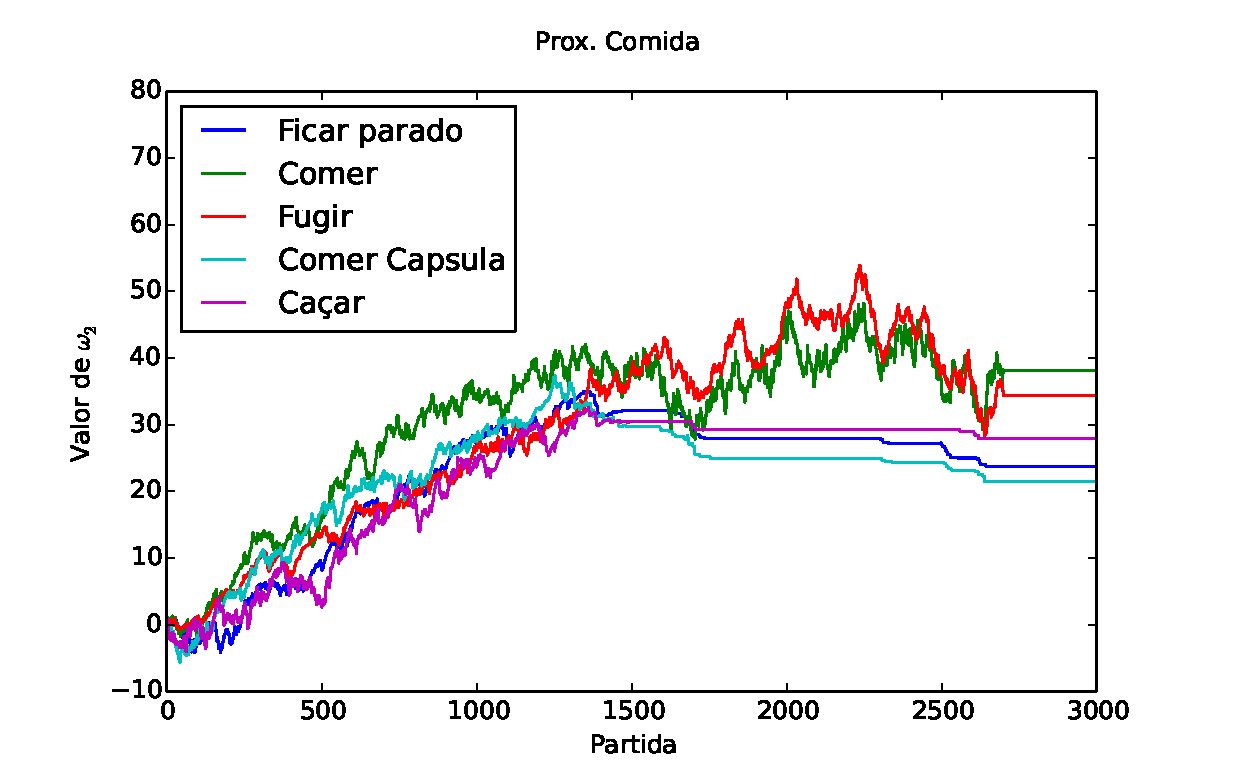
\includegraphics[width=\linewidth]{images/5_behaviors_small_map/weights____pol__DistComida}
    \caption{Evolução dos pesos $ \omega_2 $ da característica Distância para Comida $ f_2 $.}
    \label{img:5ComportamentosMapaPequeno:PesoDistComida}
\end{figure}

\begin{figure}[H]
    \centering
    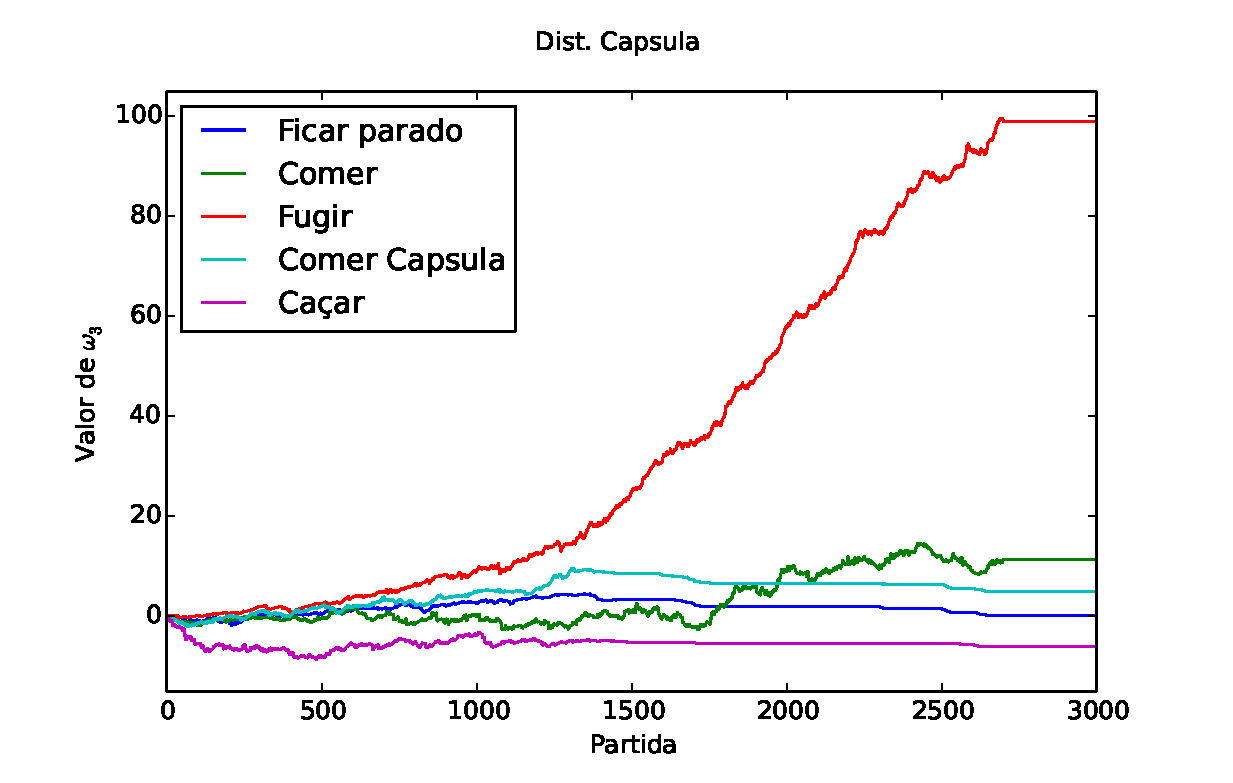
\includegraphics[width=\linewidth]{images/5_behaviors_small_map/weights____pol__DistCapsula}
    \caption{Evolução dos pesos $ \omega_3 $ da característica Distância para Cápsula $ f_3 $.}
    \label{img:5ComportamentosMapaPequeno:PesoDistCapsula}
\end{figure}

\begin{figure}[H]
    \centering
    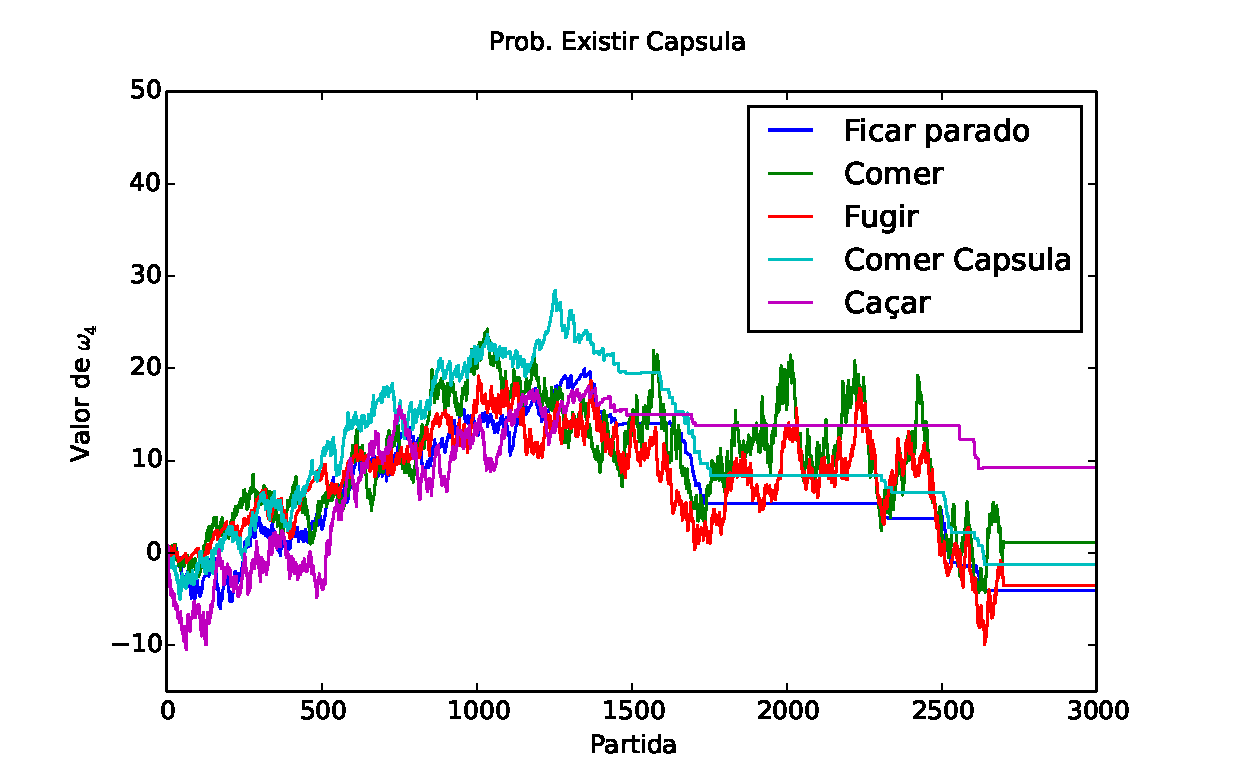
\includegraphics[width=\linewidth]{images/5_behaviors_small_map/weights____pol__ProbExistirCapsula}
    \caption{Evolução dos pesos $ \omega_4 $ da característica Probabilidade de uma Cápsula ainda Existir $ f_4 $.}
    \label{img:5ComportamentosMapaPequeno:PesoProbCapsulaExistir}
\end{figure}

\begin{figure}[H]
    \centering
    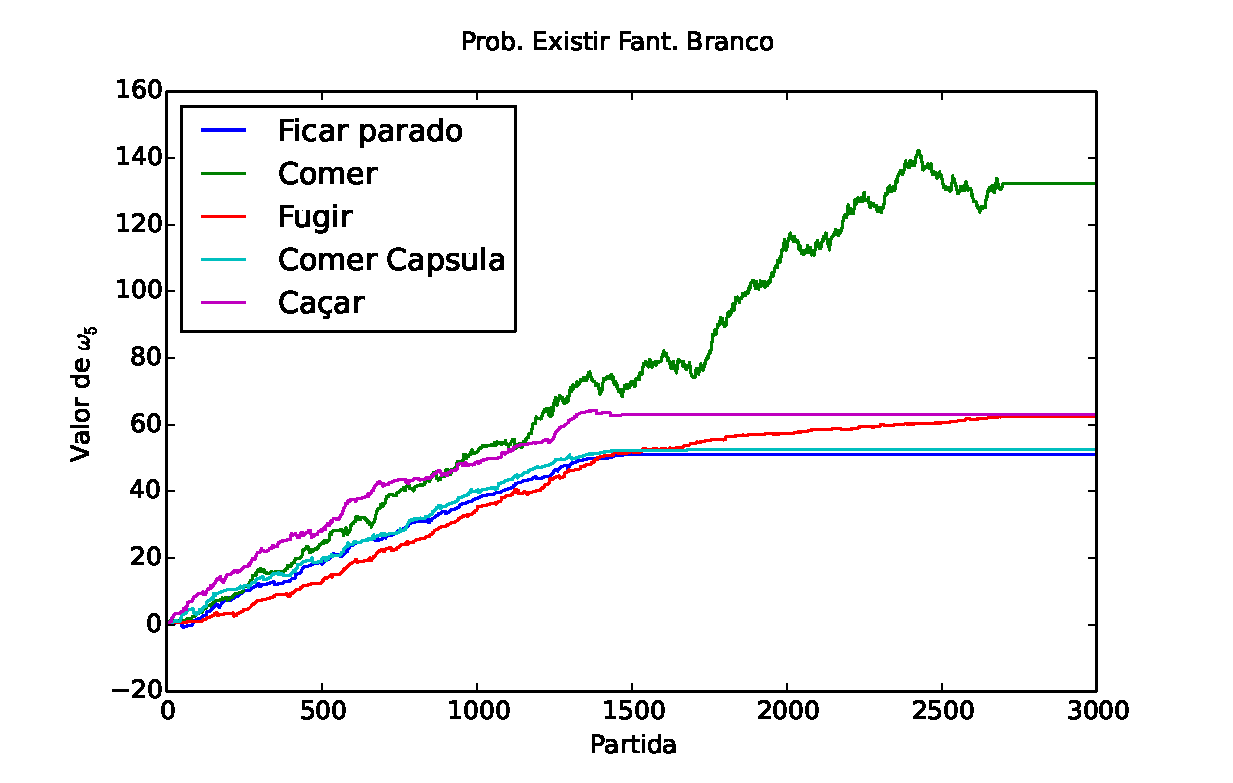
\includegraphics[width=\linewidth]{images/5_behaviors_small_map/weights____pol__ProbExistirFantBranco}
    \caption{Evolução dos pesos $ \omega_5 $ da característica Probabilidade de Fantasma Branco Existir $ f_5 $.}
    \label{img:5ComportamentosMapaPequeno:PesoProbFantasmaBrancoExistir}
\end{figure}

\begin{figure}[H]
    \centering
    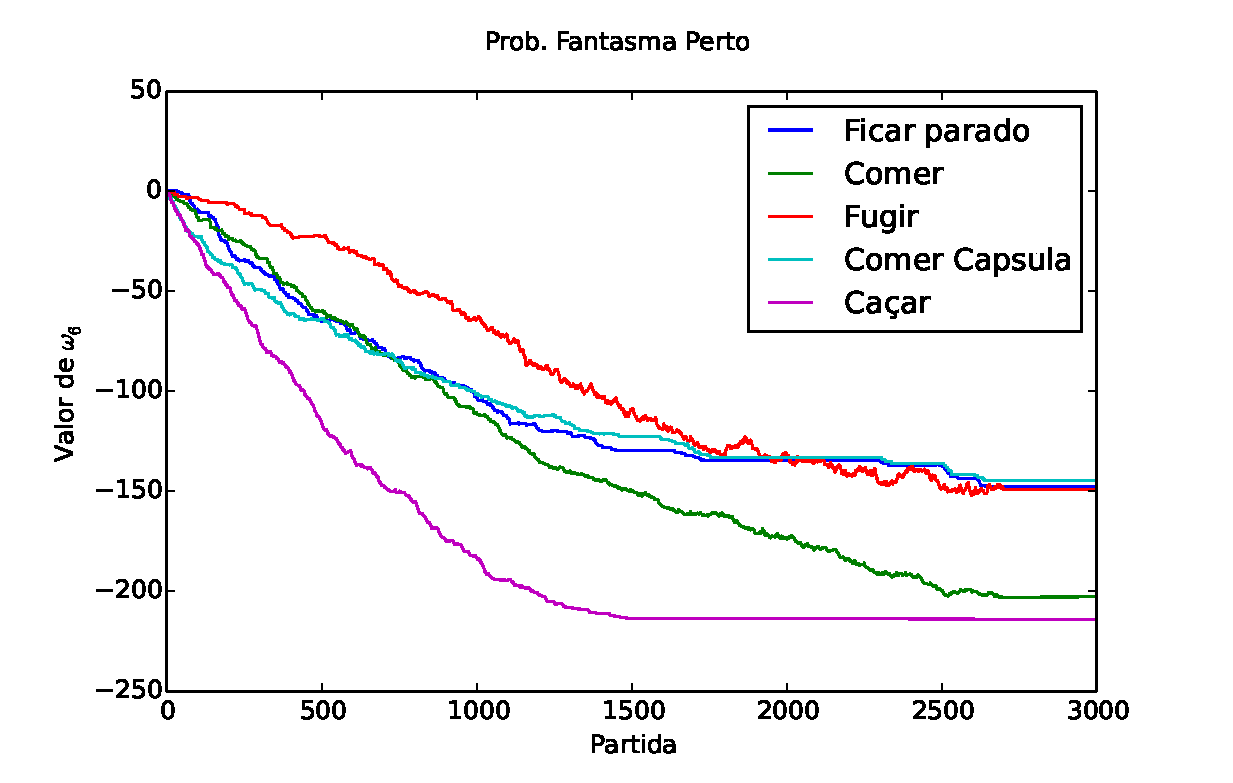
\includegraphics[width=\linewidth]{images/5_behaviors_small_map/weights____pol__ProbFantasmaPerto}
    \caption{Evolução dos pesos $ \omega_6 $ da característica Probabilidade de Fantasma por Perto $ f_6 $.}
    \label{img:5ComportamentosMapaPequeno:PesoProbFantasmaPorPerto}
\end{figure}

\begin{figure}[H]
    \centering
    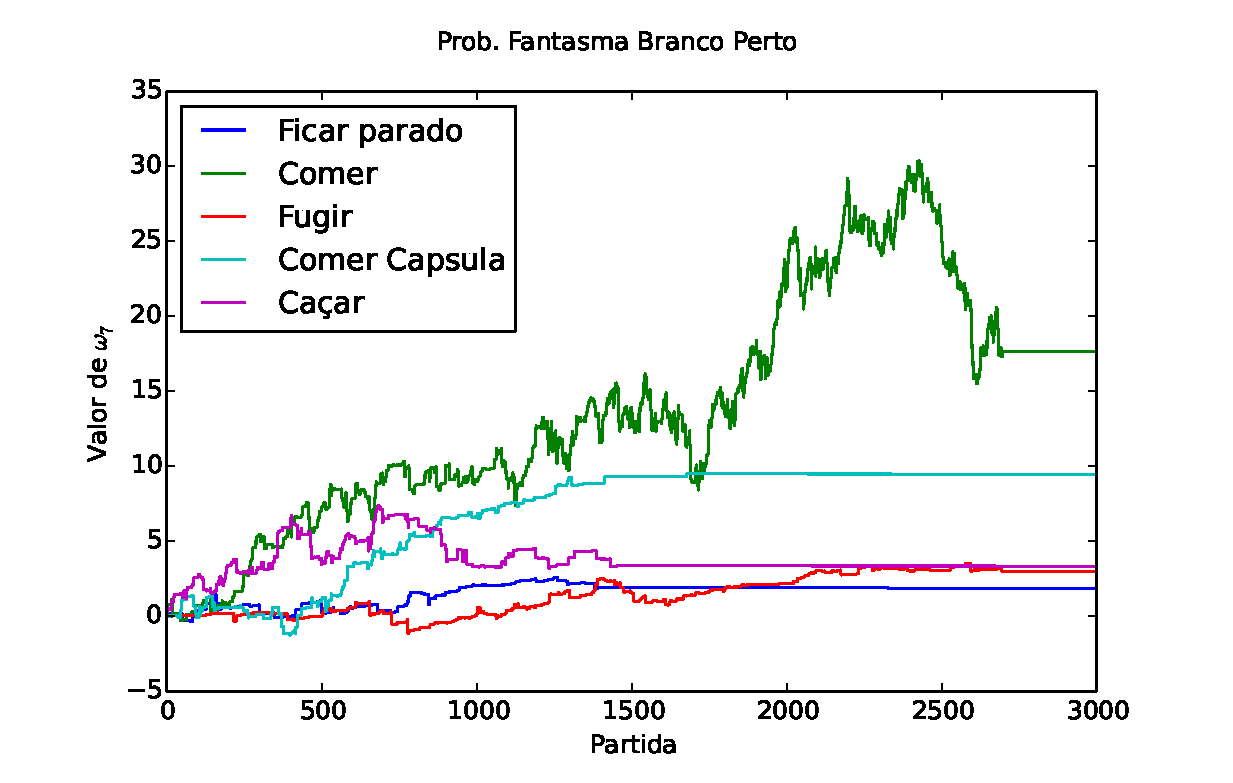
\includegraphics[width=\linewidth]{images/5_behaviors_small_map/weights____pol__ProbFantasmaBrancoPerto}
    \caption{Evolução dos pesos $ \omega_7 $ da característica Probabilidade de Fantasma Branco por Perto $ f_7 $.}
    \label{img:5ComportamentosMapaPequeno:PesoProbFantasmaBrancoPorPerto}
\end{figure}

Nesse experimento é mais difícil de fazer análise dos pesos, pois temos agora 7 pesos para comparar. Algumas características são fáceis de entender, por exemplo, ter um fantasma normal por perto é muito ruim quando se está comendo, e pior ainda quando se está caçando. Por outro lado $ Fugir $ ou $ Comer\_Capsula $ são boas alternativas nesse caso.

Para outras caracteríticas, é mais complexo entender o comportamento de seus pesos. A característica $ Prob Fantasma Branco Perto $, por exemplo, tem maior peso para $ Comer $ que para $ \textit{Caçar} $. Isso se dá, em boa parte, pela natureza probabilística do sistema. Como há uma probabilidade de esse fantasma não estar realmente branco, caçar pode não ser uma solução tão boa quanto ignorar os fantasmas e escolher o comportamento de $ Comer $.

Plotando o número de vezes que cada comportamentos é escolhido por partida para esse experimento, eles formam a nuvem exposta na figura \ref{img:5ComportamentosMapaPequeno:ComportamentosEscolhidos}.

\begin{figure}[H]
    \centering
    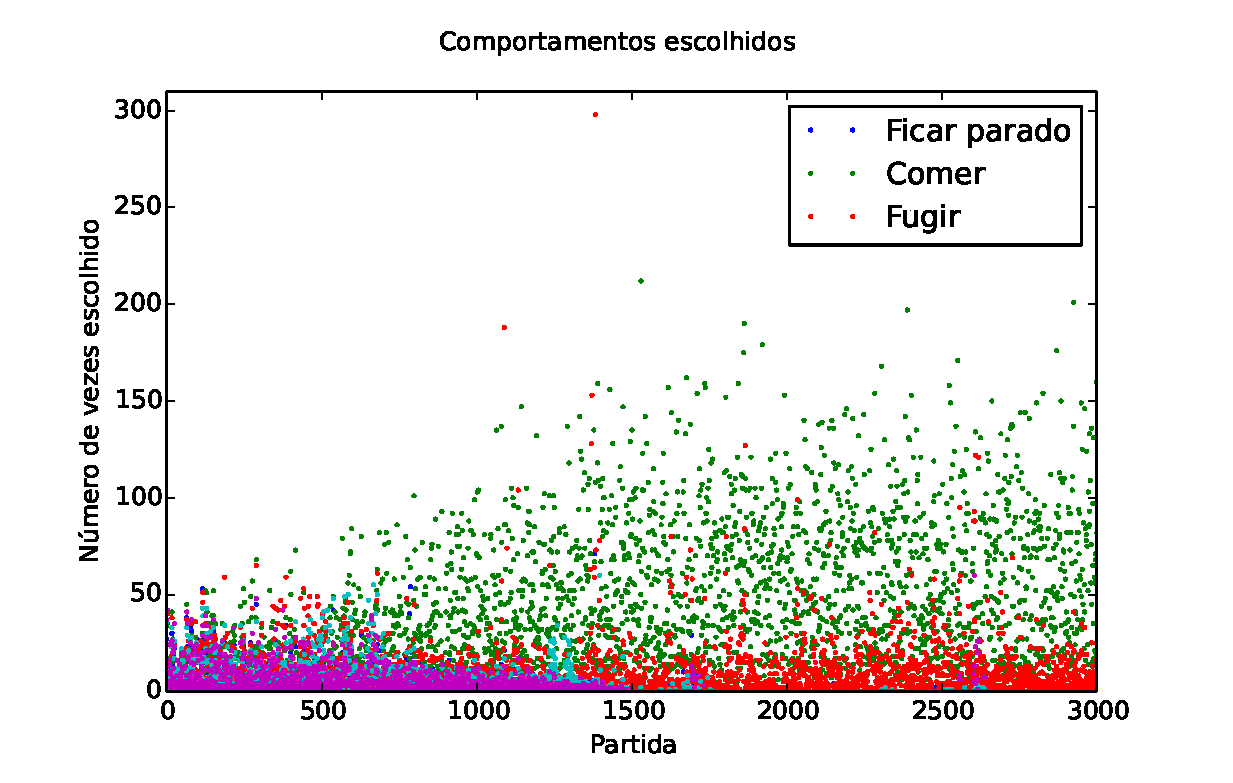
\includegraphics[width=\linewidth]{images/5_behaviors_small_map/chosen_behaviors}
    \caption{Escolha de comportamentos por partida.}
    \label{img:5ComportamentosMapaPequeno:ComportamentosEscolhidos}
\end{figure}

Novamente, para ter uma visualização melhor achamos um polinômio que represente essa nuvem de pontos, utilizando o método dos mínimos quadrados. Para um polinômio de quarto grau essa curva fica como a descrita na figura \ref{img:5ComportamentosMapaPequeno:ComportamentosEscolhidosPolinômio}.

\begin{figure}[H]
    \centering
    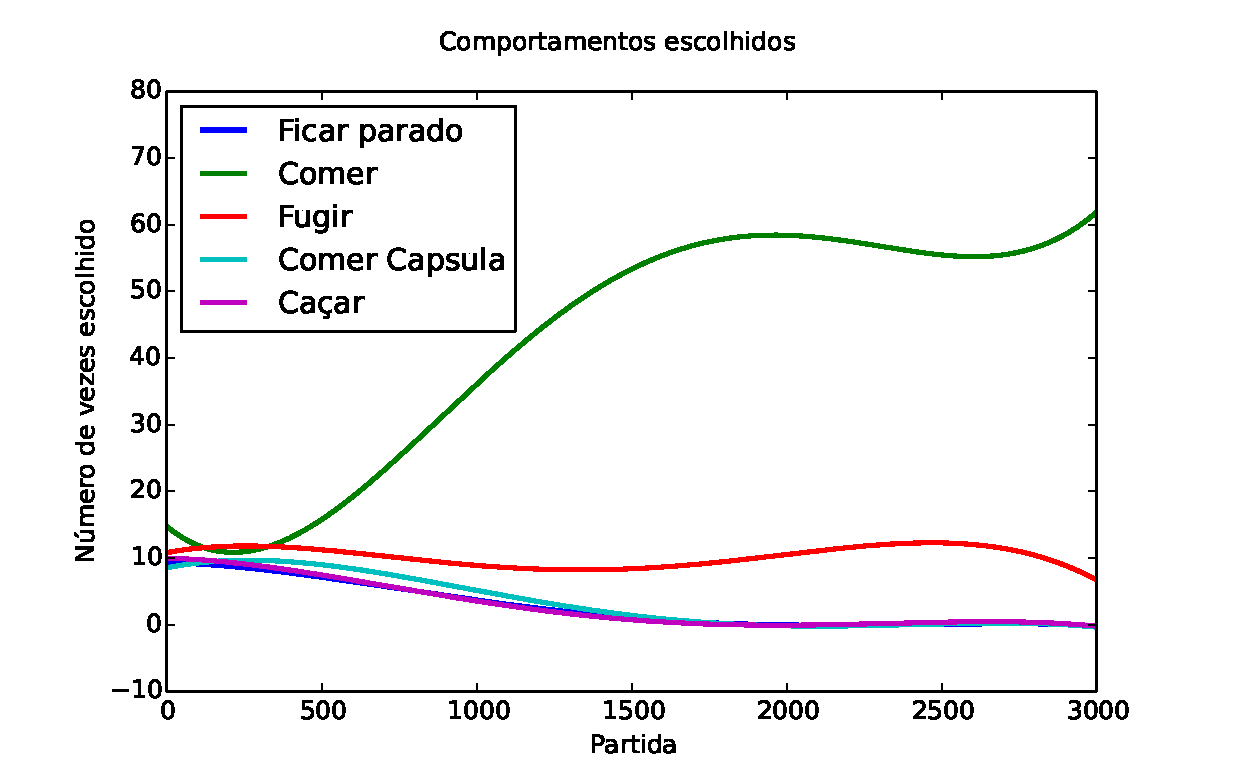
\includegraphics[width=\linewidth]{images/5_behaviors_small_map/chosen_behaviors_pol}
    \caption{Escolha de comportamentos por partida.}
    \label{img:5ComportamentosMapaPequeno:ComportamentosEscolhidosPolinômio}
\end{figure}

Nesse experimento, o comportamento $ Comer $ novamente tem o maior número de execuções, sendo $ Fugir $ o único que continua sendo executado até o final. Isso pode ser justificado por um fato não esperado, observado no experimento. O algoritmo ``percebeu'' que muitas das vezes que o comportamento $ Fugir $ é executado, o agente foge para cima da Cápsula, não só evitando o fantasma, mas servindo de substituto ao comportamento $ Comer\_Capsula $. Por isso o peso $ \omega_3 $, da característica $ Prox. Capsula $, é máximo para esse comportamento. Além disso, o comportamento $ Comer $, além de ir atrás da comida, muitas vezes acaba indo em direção a um fantasma branco nesse mapa pequeno.

A pontuação para cada partida pode ser vista na imagem à seguir, \ref{img:5ComportamentosMapaPequeno:PontuacaoPorPartida}. Novamente aproximamos esses dados por um polinômio de terceiro grau, utilizando o método dos mínimos quadrado.

\begin{figure}[H]
    \centering
    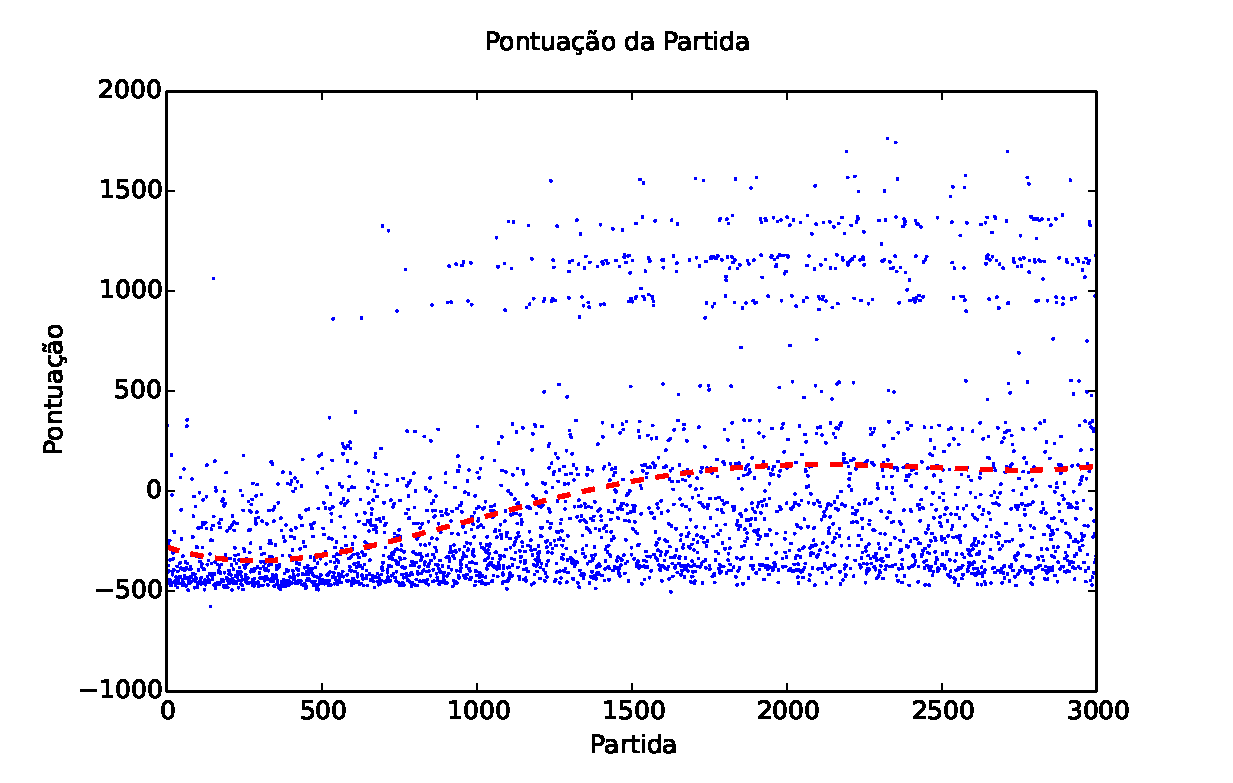
\includegraphics[width=\linewidth]{images/5_behaviors_small_map/match_scores____pol}
    \caption{Escolha de comportamentos por partida.}
    \label{img:5ComportamentosMapaPequeno:PontuacaoPorPartida}
\end{figure}

Exceto pelo inicio do experimento, aproximadamente as primeiras trezentas partidas, a pontuação aumenta durante todo o treinamento. A média de pontos feita, após a conclusão do treinamento:

$$ mean \left( score \right) = 143.93 $$

Sendo a média de escolha por partida dos comportamentos:

$$ mean \left( Ficar\_Parado \right) = 0.0 $$
$$ mean \left( Comer \right) = 59.10 $$
$$ mean \left( Fugir \right) = 8.35 $$
$$ mean \left( Comer\_Capsula \right) = 0.0 $$
$$ mean \left( \textit{Caçar} \right) = 0.0 $$


\subsection{Discussão}

O algoritmo, nesse experimento, após completo o treinamento, escolheu somente os comportamentos $ Comer $ e $ Fugir $, mesmo em posse dos outros. Isso pode ser explicado, em parte devido a particularidades encontradas no mapa, que não eram esperadas a princípio, e em parte pela natureza probabilística do sistema, o que dificulta se ter uma certeza de os fantasmas estarem brancos.


\section{5 Comportamentos no mapa original (Teste 4)}


\section{Discussão Geral}

O algoritmo, como esperado, teve comportamentos diferentes, para diferentes mapas, comportamentos e parâmetros.

Algumas coisas inesperadas foram observadas, por exemplo, no terceiro caso de teste, mesmo só executando, ao final, dois comportamentos, $ Comer $ e $ Fugir $, os mesmo executados pelo primeiro experimento, ele conseguiu uma média de pontos bastante superior. Isso se deve ao caso de uma característica, que parecia ter pouca relevância para esses dois comportamentos, ser mais importante que o esperado. Isso reforça a informação dada na Fundamentação Teórica, no tópico \ref{subsection:GeneralizaçãoParesEstadoAção}, que falava ``devemos escolher esses valores/características com cuidado para obter uma boa representação do nosso par estado-ação [...] ou podemos ter estados-ações com valores [...] parecidos, e, consequentemente, valores de $ Q \left( S, U \right) $ também parecidos, mas que são muito diferentes.''

Mesmo com alguns acontecimentos diferentes, de modo geral o algoritmo se comportou como se esperava. Nos experimentos com o mapa clássico, por exemplo, ele aprende e valoriza muito mais a ação de comer, enquanto nos mapas pequenos ele é muito mais cauteloso.

O modelo obteve bons resultados, conseguindo fazer escolhas satisfatórias mesmo num sistema com alto erro de atuação e sensoriamento e sem ter nenhuma informação previa de como os comportamentos influenciariam seu desenpenho ou atuação.






--------------------------------------------

--------------------------------------------

--------------------------------------------

--------------------------------------------

--------------------------------------------


Falar da independencia comida-posicao

Ajeitar Gráficos e Texto - Proximidade da Comida e da Cápsula no lugar de Distância